\documentclass[12pt,aspectratio=169]{beamer}

\usepackage{minted}

\usetheme[progressbar=frametitle, numbering=fraction]{metropolis}
\usepackage{appendixnumberbeamer}

\usepackage{booktabs}
\usepackage[scale=2]{ccicons}

\usepackage{pgfplots}
\usepgfplotslibrary{dateplot}

\usepackage{xspace}
\newcommand{\themename}{\textbf{\textsc{metropolis}}\xspace}

% Chinese Fonts (Fontset: fandol,ubuntu)
\usepackage[fontset=fandol]{ctex}

% Math Fonts
\usefonttheme{professionalfonts} 
\usepackage{mathspec}
% \setsansfont[BoldFont={Fira Sans},Numbers={OldStyle}]{Fira Sans Light}
% \setmathsfont(Digits)[Numbers={Lining, Proportional}]{Fira Sans Light}

% Change Color of the theme
\usepackage{xcolor}
\definecolor{DarkGrey}{HTML}{353535}
\definecolor{ECNURed}{RGB}{164,31,53}
\definecolor{ECNUBrown}{RGB}{134,117,77}
\setbeamercolor{normal text}{ fg= DarkGrey  }
\setbeamercolor{alerted text}{ fg= ECNURed  }
\setbeamercolor{example text}{ fg= ECNUBrown  }

% Bolder Fonts for presenting in a large room 
\setsansfont[BoldFont={Fira Sans SemiBold}]{Fira Sans Book}

\title{搜索算法}
\subtitle{深度优先与广度优先搜索}
\date{\today}
\author{罗江楠}
\institute{哈尔滨工业大学(威海)}
\titlegraphic{\hfill
\includegraphics[height=1cm]{hitwh.png}}

\begin{document}

\maketitle

\begin{frame}{目录}
  \setbeamertemplate{section in toc}[sections numbered]
  \tableofcontents[hideallsubsections]
\end{frame}

\section[引言]{Introduction}

\begin{frame}[fragile]{引言}
  其实我也不知道要说什么\pause

  就祝大家新年快乐吧
\end{frame}

\section[深度优先搜索]{Depth First Search}

\begin{frame}[fragile]{深度优先搜索}
  \begin{itemize}
    \item 尽可能深地搜索树的分支
    \item 直到所有可能情况都被完全搜索一遍
  \end{itemize}
\end{frame}

\begin{frame}[fragile]{例题:整数分解}
  \begin{itemize}
    \item 求解有多少种将正整数 $n$ 分解为 $3$ 个正整数相加的方案
    \item 两种分解方案不同当且仅当加数中的其中一个数字不相同
    \item 例如 $4=1+1+2=1+2+1=2+1+1$ 共有 $3$ 种不同的分解方式
  \end{itemize}
\end{frame}

\begin{frame}[fragile]{例题:整数分解}
  考虑你们之前学过的枚举算法
  \begin{verbatim}
for (int i = 1; i <= n; ++ i)
  for (int j = 1; j <= n; ++ j)
    for (int k = 1; k <= n; ++ k)
      if (i + j + k == n)
        printf("%d = %d + %d + %d\n", n, i, j, k);
  \end{verbatim}\pause
  时间复杂度 $O(n^3)$
\end{frame}

\begin{frame}[fragile]{例题:整数分解}
  可以考虑优化枚举的上下界,可以将复杂度降低到 $O(n^2)$
  \begin{verbatim}
for (int i = 1; i <= n - 2; ++ i)
  for (int j = 1; j <= n - i - 1; ++ j)
    printf("%d = %d + %d + %d\n", n, i, j, n - i - j);
  \end{verbatim}
\end{frame}

\begin{frame}[fragile]{例题:整数分解}
  \begin{itemize}
    \item 但是如果将题目改成分解成 $4$ 个正整数的和呢?\pause
    \item 写 $4$ 重 \verb|for| 循环?\pause
    \item 如果改成 $m$ 个正整数呢?\pause
    \item 写 $m$ 重 \verb|for| 循环?\pause
    \item 此时就需要运用这个被称为\textbf{深度优先搜索}的算法了
  \end{itemize}
\end{frame}

\begin{frame}[fragile]{深度优先搜索算法}
  深度优先搜索算法一般使用递归的算法,遵从以下流程
  \begin{itemize}
    \item 首先判断搜索的当前状态是否满足\textbf{结束条件}
    \item 如果结束满足则输出当前状态并返回
    \item 接下来考虑枚举当前状态的每一个可能的下一个状态的转移
    \item 将该转移应用到当前的状态中
    \item 向下递归搜索
    \item 将当前状态恢复为转移前的状态
  \end{itemize}
\end{frame}

\begin{frame}[fragile]{例题:整数分解}
  \begin{minted}{cpp}
int ans[100]; // 用于储存当前分解方案的数组
void dfs(int x, int k) { // 将 x 分解成 k 个正整数
  if (k == 1) { // 搜索的结束条件
    ans[k] = x; output(ans); // 输出方案
    return;
  }
  for (int i = 1; i <= x - k + 1; ++ i) {
    ans[k] = i; // 记录方案
    dfs(x - i, k - 1); // 递归搜索
  }
}
  \end{minted}
\end{frame}

\begin{frame}[fragile]{例题:整数分解}
  \begin{figure}
    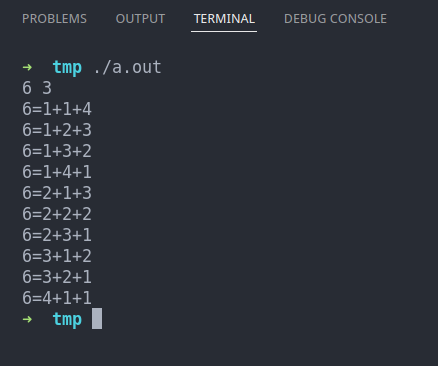
\includegraphics[height=200pt]{example1.png}
  \end{figure}
\end{frame}

\begin{frame}[fragile]{例题:八皇后问题}
  如何能够在 $8 \times 8$ 的国际象棋棋盘上放置八个皇后,使得任何一个皇后都无法直接吃掉其他的皇后?

  \begin{figure}
    
\includegraphics[height=100pt]{killer_queen.jpeg}
    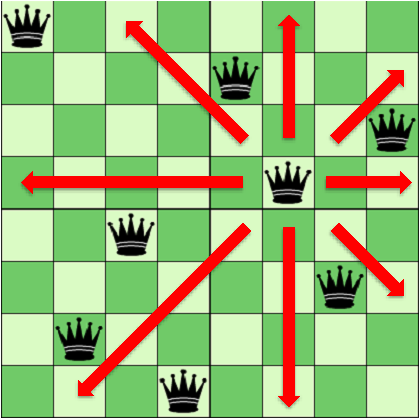
\includegraphics[height=100pt]{queen.png}
  \end{figure}
\end{frame}

\subsection[剪枝优化]{Decision Tree Pruning}

\section[广度优先搜索]{Breadth First Search}
\subsection[堆优化]{Heap Optimization}

\section[例题]{Examples}

\end{document}